\documentclass[12pt
,headinclude
,headsepline
,bibtotocnumbered
]{scrartcl}
\usepackage[paper=a4paper,left=25mm,right=25mm,top=25mm,bottom=25mm]{geometry} 
\usepackage[utf8]{inputenc}
\usepackage[english]{babel}
\usepackage{fancyvrb}  % Add this line
\usepackage{graphicx}
\usepackage{multirow}
\usepackage{pdfpages}
%\usepackage{wrapfig}
\usepackage{placeins}
\usepackage{float}
\usepackage{flafter}
\usepackage{mathtools}
\usepackage{hyperref}
\usepackage{epstopdf}
\usepackage[miktex]{gnuplottex}
\usepackage[T1]{fontenc}
\usepackage{mhchem}
\usepackage{fancyhdr}
%\setlength{\mathindent}{0pt}
\usepackage{amssymb}
\usepackage[list=true, font=large, labelfont=bf, 
labelformat=brace, position=top]{subcaption}
\setlength{\parindent}{0mm}
\usepackage{listings}
\usepackage{color}

\definecolor{dkgreen}{rgb}{0,0.6,0}
\definecolor{gray}{rgb}{0.5,0.5,0.5}
\definecolor{mauve}{rgb}{0.58,0,0.82}

\lstset{ %
	language=Matlab,                % the language of the code
	basicstyle=\small\ttfamily,     % the size of the fonts that are used for the code
	numbers=left,                   % where to put the line-numbers
	numberstyle=\tiny\color{gray},  % the style that is used for the line-numbers
	stepnumber=1,                   % the step between two line-numbers. If it's 1, each line will be numbered
	numbersep=5pt,                  % how far the line-numbers are from the code
	backgroundcolor=\color{white},  % choose the background color. You must add \usepackage{color}
	showspaces=false,               % show spaces adding particular underscores
	showstringspaces=false,         % underline spaces within strings
	showtabs=false,                 % show tabs within strings adding particular underscores
	frame=single,                   % adds a frame around the code
	rulecolor=\color{black},        % if not set, the frame-color may be changed on line-breaks within not-black text (e.g. commens (green here))
	tabsize=2,                      % sets default tabsize to 2 spaces
	captionpos=b,                   % sets the caption-position to bottom
	breaklines=true,                % sets automatic line breaking
	breakatwhitespace=true,         % sets if automatic breaks should only happen at whitespace
	title=\lstname,                 % show the filename of files included with \lstinputlisting; also try caption instead of title
	keywordstyle=\color{blue},      % keyword style
	commentstyle=\color{dkgreen},   % comment style
	stringstyle=\color{mauve},      % string literal style
	escapeinside={\%*}{*)},         % if you want to add LaTeX within your code
	morekeywords={*,...}            % if you want to add more keywords to the set
}

\setlength{\parindent}{0mm}

\pagestyle{fancy}
\fancyhf{}
\lhead{Orbit Mechanics\\ Exercise 2: Numericial Integration of Satellite Orbits}
\rhead{Hsin-Feng Ho \\03770686}
\rfoot{Page \thepage}	
\begin{document}
\begin{titlepage}
    \vspace{\fill}
    \title{\textbf{Orbit Mechanics \\ Exercise 2: Numericial Integration of Satellite Orbits}}
    \vspace{5cm}
    \author{Hsin-Feng Ho\\
    03770686}
    \vspace{3cm}
    \maketitle
\end{titlepage}
\section*{Introduction}
In the first exercise we have seeen that the orbit of a satellite can be calculated by an analytical solution of the two-body problem. The satellite orbit can also be determined by numerical integration of the equations of motion.
\\\\
The Keplerian elements for the Sentinel-3 satellite is given:
\begin{table}[H]
\centering
\renewcommand\arraystretch{1.5}
\setlength{\tabcolsep}{5mm}{
\begin{tabular}{|c|c|c|c|c|c|c|}
    \hline
    \textbf{Satellite}& \textbf{a[km]}&\textbf{e}&\textbf{i[deg]}&\textbf{$\boldsymbol{\Omega}$[deg]}&\textbf{$\boldsymbol{\omega}$[deg]}&\textbf{$\boldsymbol{T_0}$[s]}\\\hline
    Sentinel-3&7192&0.004&98.3&257.7&144.2&00:00\\\hline
\end{tabular}
}
\end{table}
\section*{Undisturbed Orbit}
Using the given Keplerian elements and analytical solution of two body problem we can calculate the orbit of the Sentinel-3 satellite. 
\begin{figure}[H]
\centering
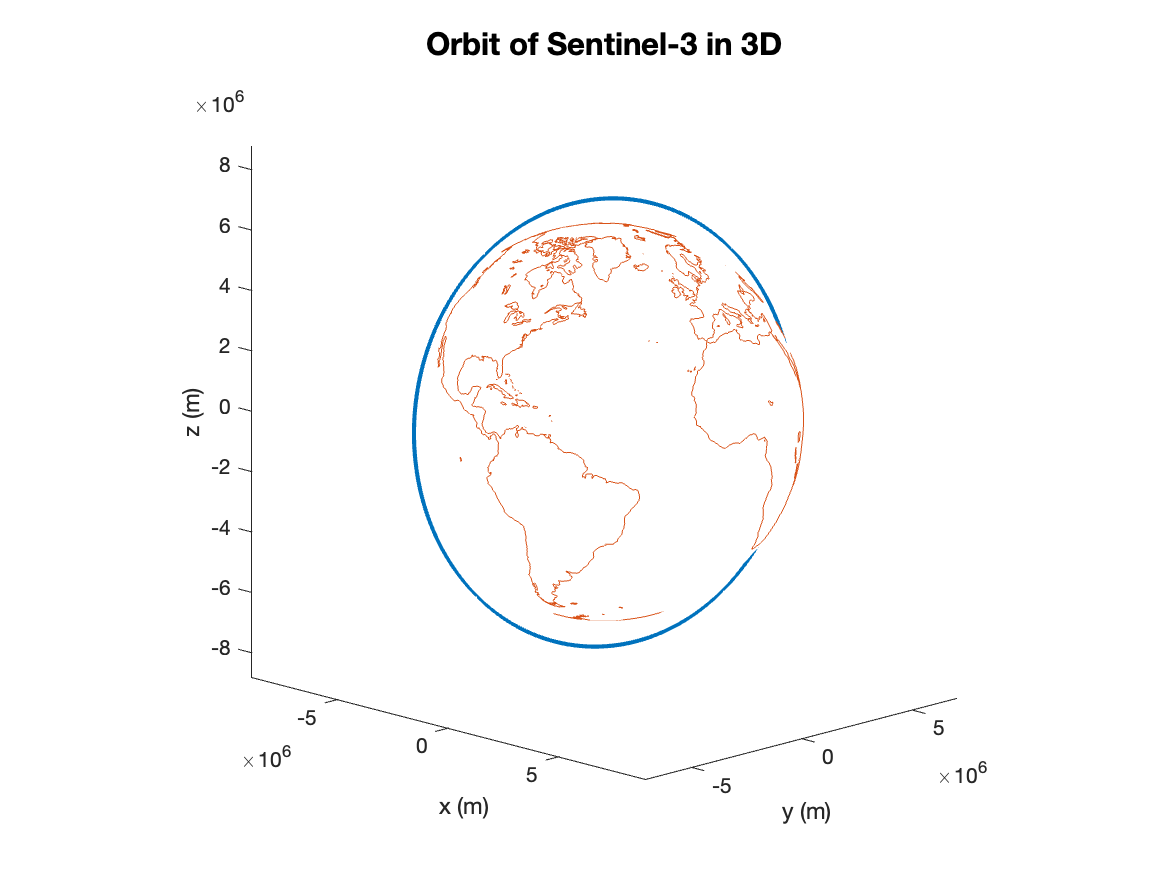
\includegraphics[width=0.8\textwidth]{./plots/3D_orbit.png}
\caption{undisturbed orbit of Sentinel-3 satellite for 3 revolutions}
\end{figure}
Now we have to calculate the satellite orbit using numerical integration. The 2nd order differential equation for the two-body problem is:
\begin{align*}
	\ddot{\textbf{r}}_i=-\frac{GM}{\left|\left|\textbf{r}_i\right|\right|^3}\textbf{r}_i
\end{align*}
where $G$ is the gravitational constant, $M$ is the mass of the Earth and $\textbf{r}_i$ is the position vector of the satellite. The equations of motion can be written as a system of first order differential equations:
\begin{align*}
	\begin{pmatrix}
	v_x\\v_y\\v_z
	\end{pmatrix}&=\begin{pmatrix}
	\dot{r_x}\\\dot{r_y}\\\dot{r_z}
	\end{pmatrix}\\
	\begin{pmatrix}
	\dot{v_x}\\\dot{v_y}\\\dot{v_z}
	\end{pmatrix}&=-\frac{GM}{R^3}\begin{pmatrix}
	r_x\\r_y\\r_z
	\end{pmatrix}
\end{align*}
where $R=\sqrt{r_x^2+r_y^2+r_z^2}$.
\\\\
Matlab offers several numerical integration functions. Now we want to compare the function \textbf{ode23} and \textbf{ode45} with step size of 5 and 50. The results are shown in the following figures:
\begin{figure}[H]
\centering
\begin{subfigure}[b]{0.45\textwidth}
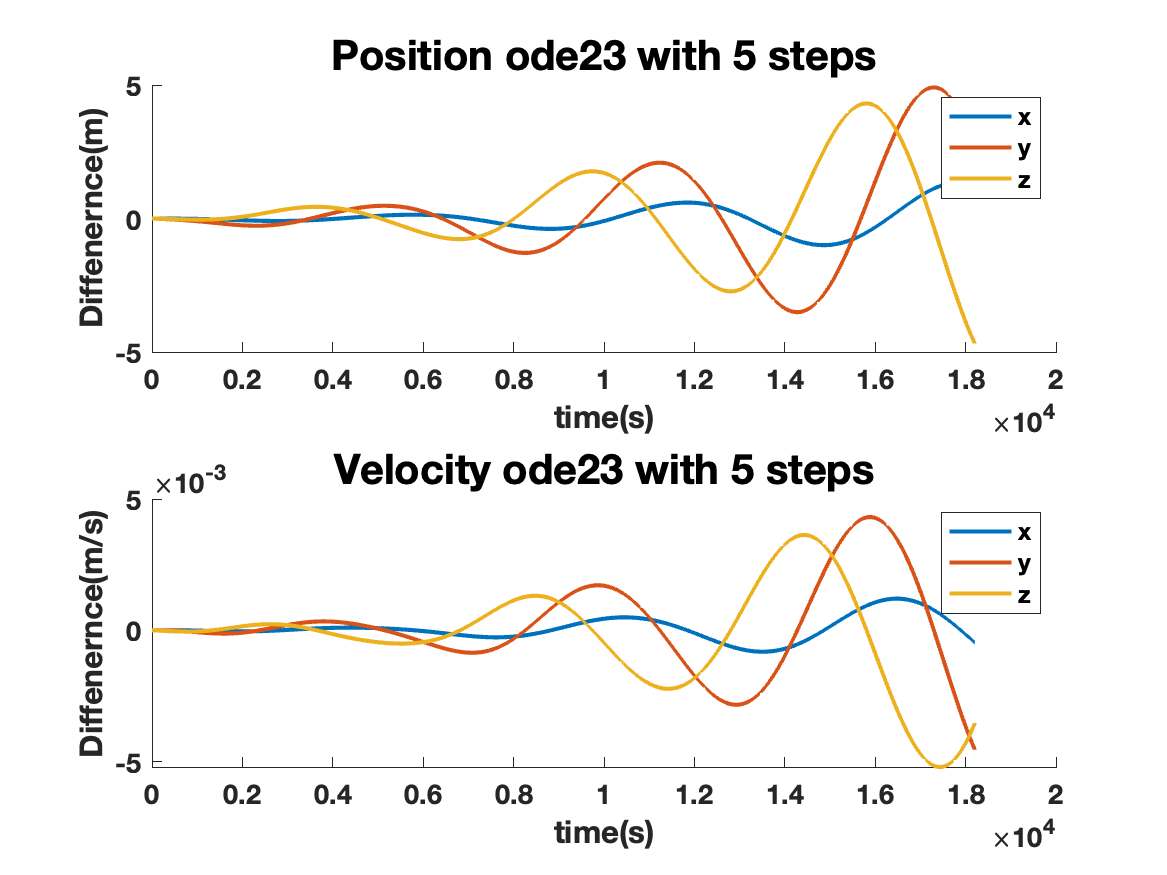
\includegraphics[width=1\textwidth]{./plots/ode23_5_yprime.png}
\end{subfigure}
\begin{subfigure}[b]{0.45\textwidth}
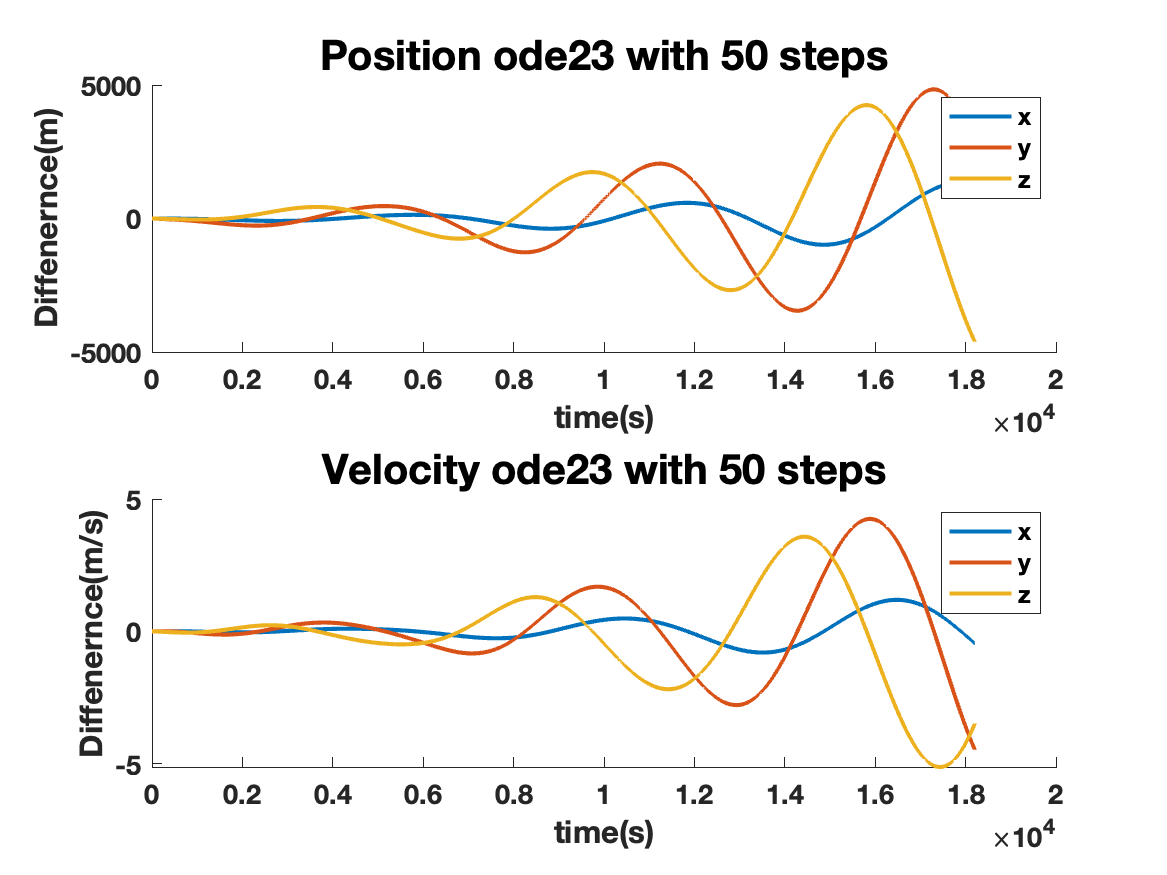
\includegraphics[width=1\textwidth]{./plots/ode23_50_yprime.png}
\end{subfigure}
\begin{subfigure}[b]{0.45\textwidth}
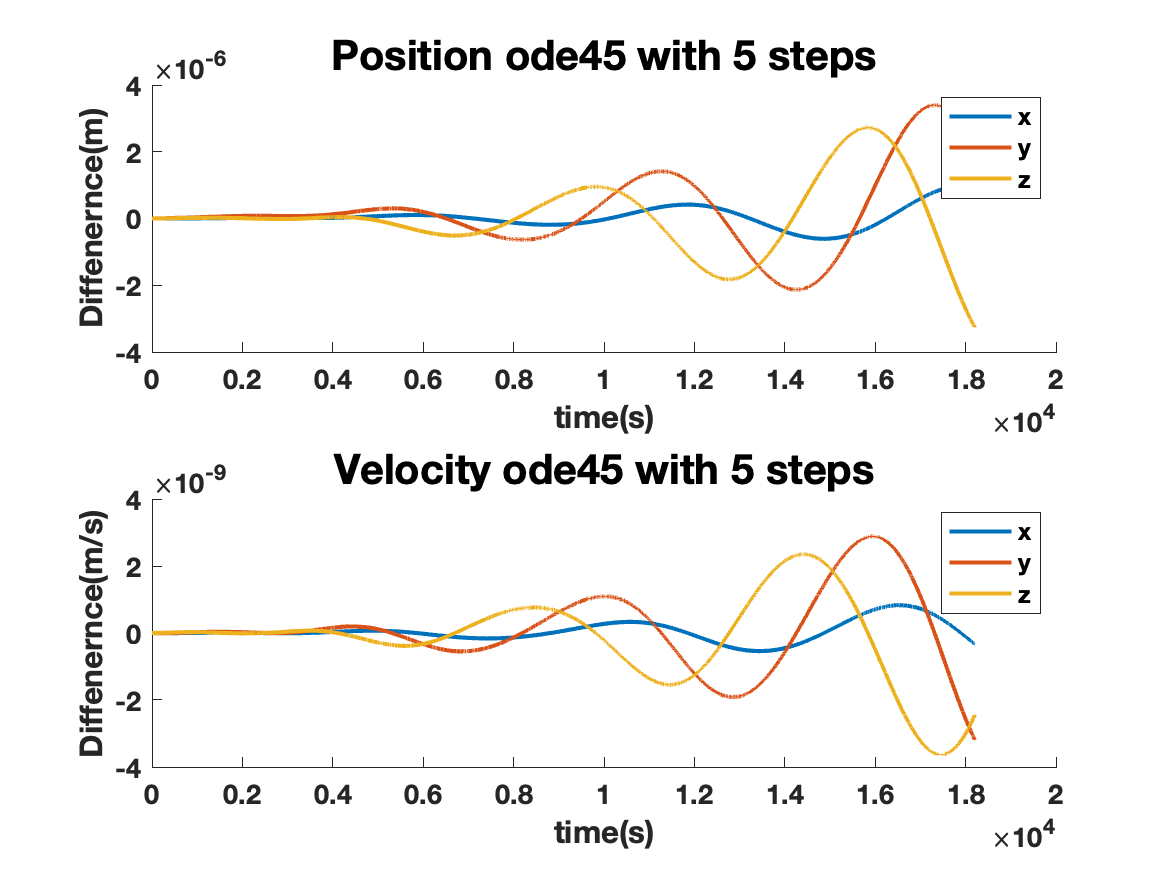
\includegraphics[width=1\textwidth]{./plots/ode45_5_yprime.png}
\end{subfigure}
\begin{subfigure}[b]{0.45\textwidth}
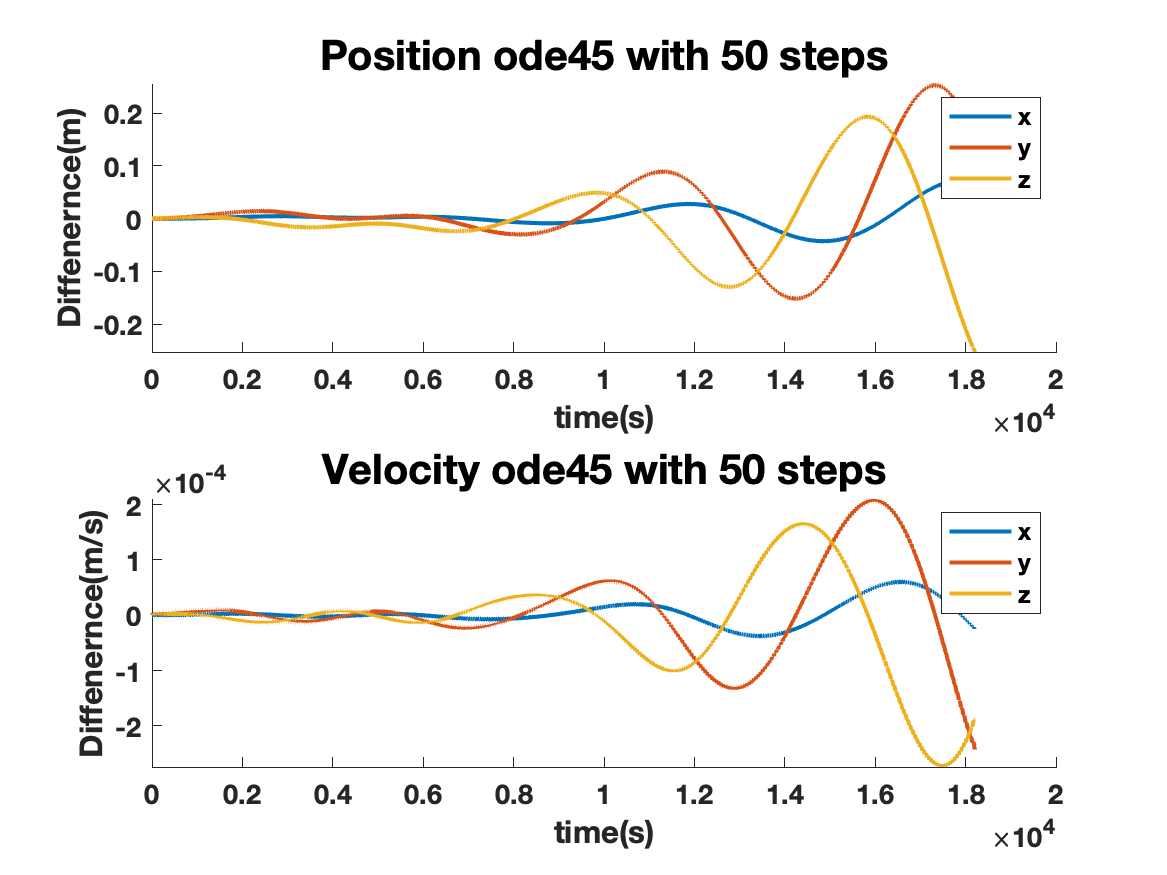
\includegraphics[width=1\textwidth]{./plots/ode45_50_yprime.png}
\end{subfigure}
\end{figure}
By observing the figures we can see that \textbf{ode45} is more accurate than \textbf{ode23}. The smaller the step size is, the more accurate the result is. The result of \textbf{ode45} with step size of 5 can even reach a precision of $10^{-6}$m in position. In comparison, the result of \textbf{ode23} with step size of 5 is only accurate to meter level in position. With step size of 50, the result of \textbf{ode23} has a difference of 5km position and 5m/s velocity compared to the analytical solution, which we should avoid in practice.
\subsection*{Decomposition of the Error in RSW system}
The error of the numerical integration can be decomposed into radial, along-track and cross-track directions in the RSW system. The radial direction is the direction from the satellite to the center of the Earth. The along-track direction is the direction of the velocity vector of the satellite. The cross-track direction is the direction perpendicular to the radial and along-track directions. The error in the RSW system can be calculated by:
\begin{align*}
    \textbf{e}_R=\frac{\textbf{r}}{|\textbf{r}|}\qquad\textbf{e}_W=\frac{\textbf{r}\times\textbf{v}}{|\textbf{r}\times\textbf{v}|}\qquad\textbf{e}_S=\textbf{e}_W\times\textbf{e}_R\\
    \Delta r_R=\textbf{e}_R\cdot\Delta\textbf{r}\qquad\Delta r_W=\textbf{e}_W\cdot\Delta\textbf{r}\qquad\Delta r_S=\textbf{e}_S\cdot\Delta\textbf{r}
\end{align*}
The results are shown in the following figures:
\begin{figure}[H]
    \centering
    \begin{subfigure}[b]{0.45\textwidth}
    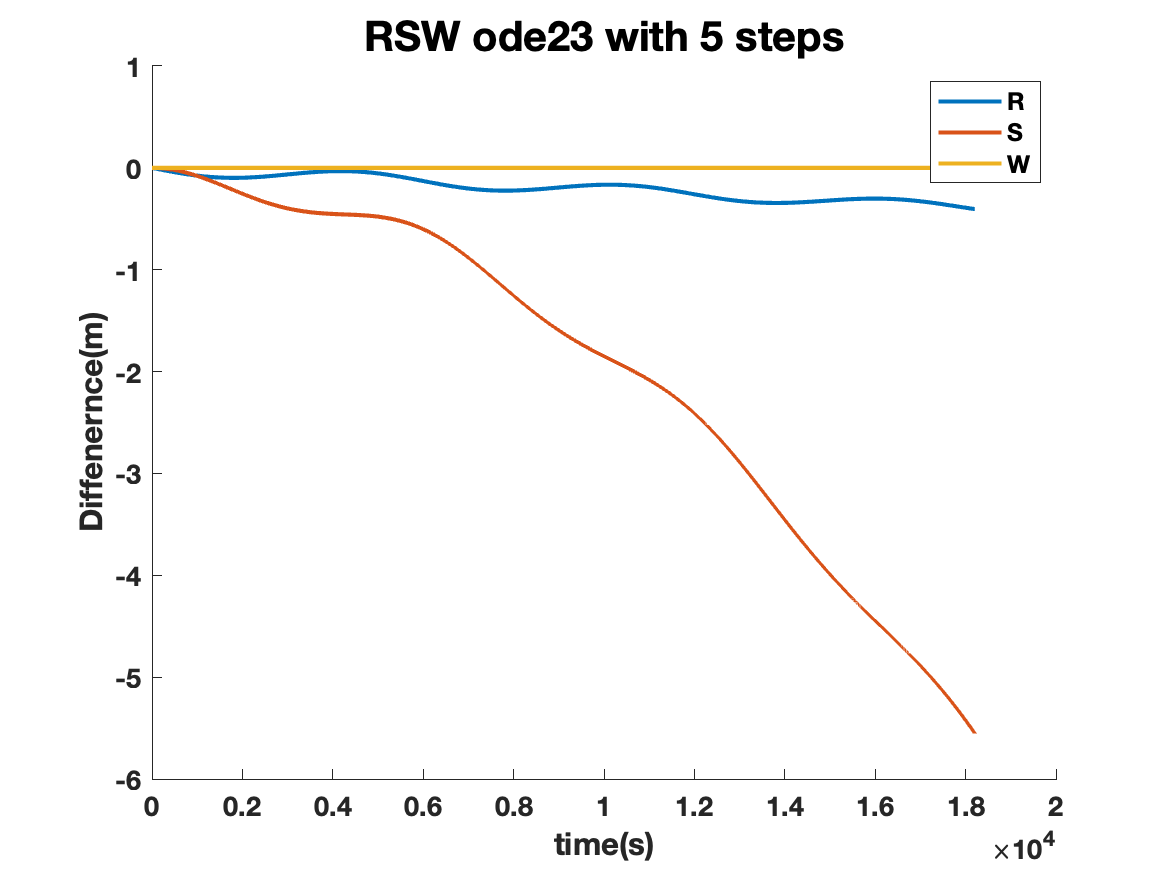
\includegraphics[width=1\textwidth]{./plots/ode23_5_yprime_RSW.png}
    \end{subfigure}
    \begin{subfigure}[b]{0.45\textwidth}
    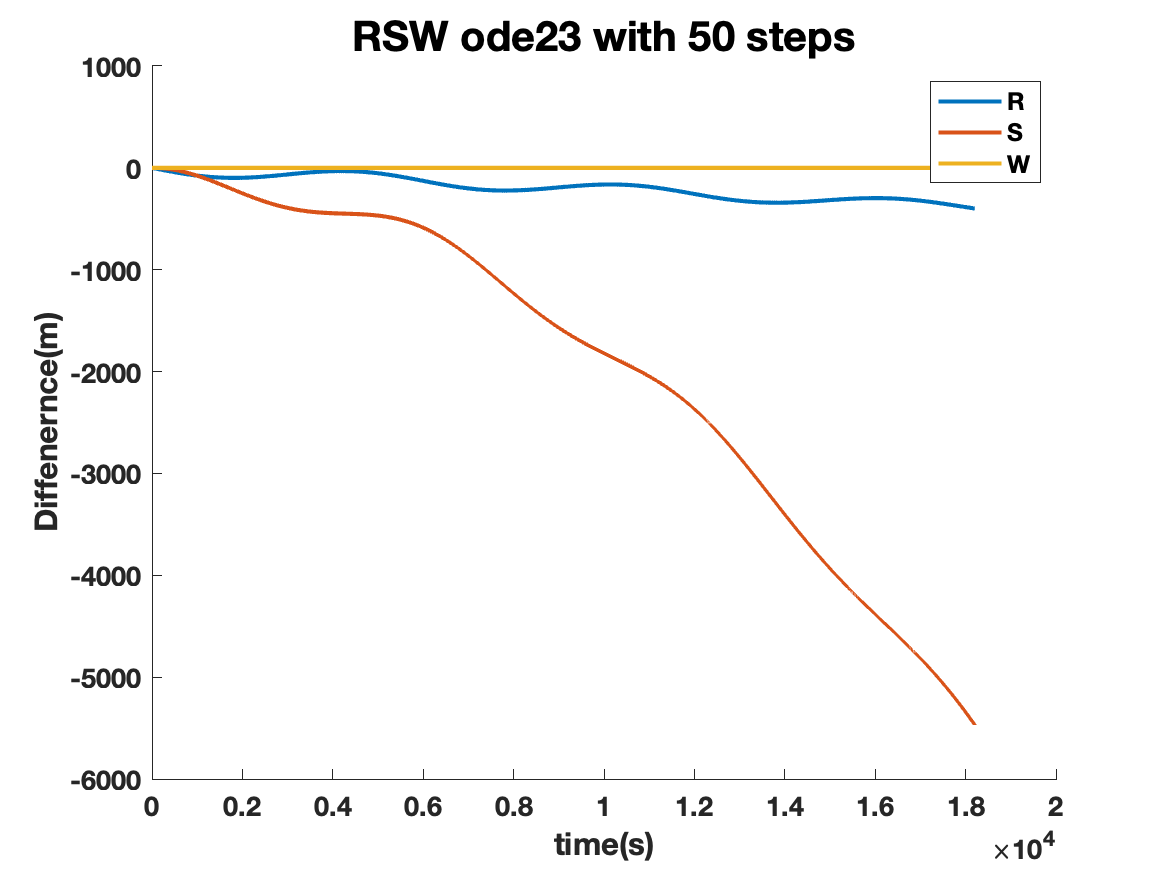
\includegraphics[width=1\textwidth]{./plots/ode23_50_yprime_RSW.png}
    \end{subfigure}
    \begin{subfigure}[b]{0.45\textwidth}
    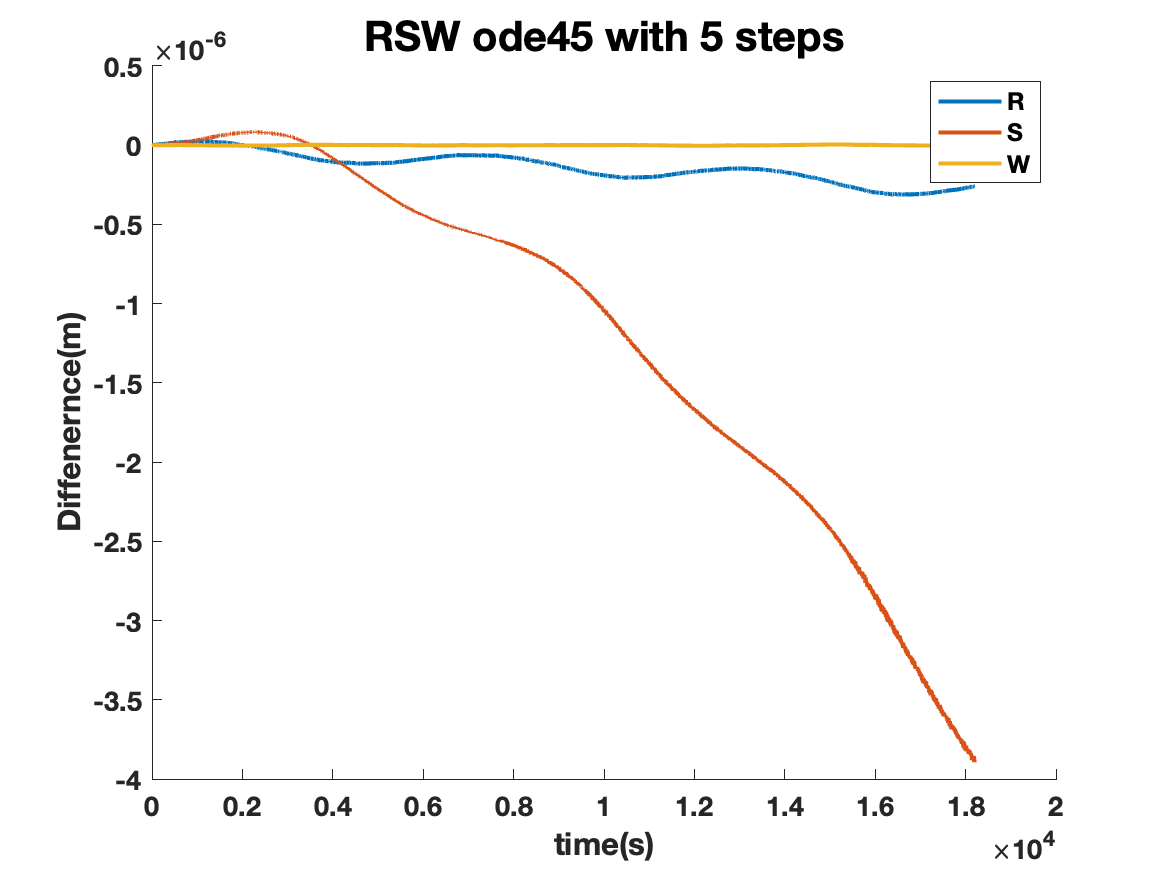
\includegraphics[width=1\textwidth]{./plots/ode45_5_yprime_RSW.png}
    \end{subfigure}
    \begin{subfigure}[b]{0.45\textwidth}
    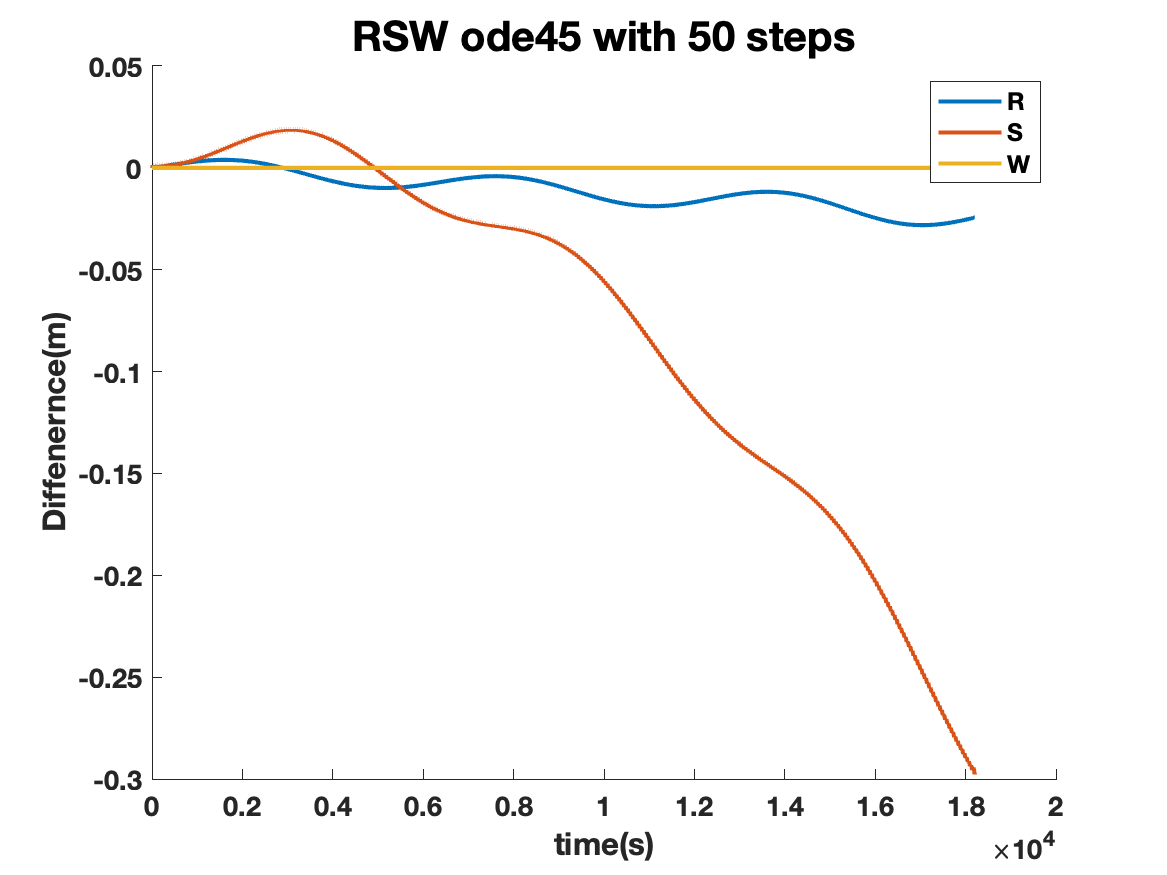
\includegraphics[width=1\textwidth]{./plots/ode45_50_yprime_RSW.png}
    \end{subfigure}
    \end{figure}
    We can see that the error is mostly in the along-track (S) direction. The error in the radial (R) and cross-track (W) directions are relatively small. Compare the two different step sizes, we can see that the error in the radial direction is smaller with smaller step size. 
    \section*{Disturbed Orbit}
    Now we want to add the perturbation of the Earth's oblateness to the equations of motion. The perturbation of the Earth's oblateness is given by:
    \begin{equation*}
        \ddot{\textbf{r}}_i=-\frac{GM}{r^3}\textbf{r}_i+\frac{3}{2}\frac{J_2a_e^2}{r^2}\begin{pmatrix}
            x\left(5\left(\frac{z}{r}\right)^2-1\right)\\
            y\left(5\left(\frac{z}{r}\right)^2-1\right)\\
            z\left(5\left(\frac{z}{r}\right)^2-3\right)
        \end{pmatrix}
    \end{equation*}
    where $J_2$ is the harmonic coefficient describing Earth oblateness, $a_e$ is the equatorial radius of the Earth and $r=\sqrt{x^2+y^2+z^2}$.
    \\\\
    The results of the numerical integration with the perturbation of the Earth's oblateness are shown in the following figures:
    \begin{figure}[H]
        \centering
        \begin{subfigure}[b]{0.45\textwidth}
        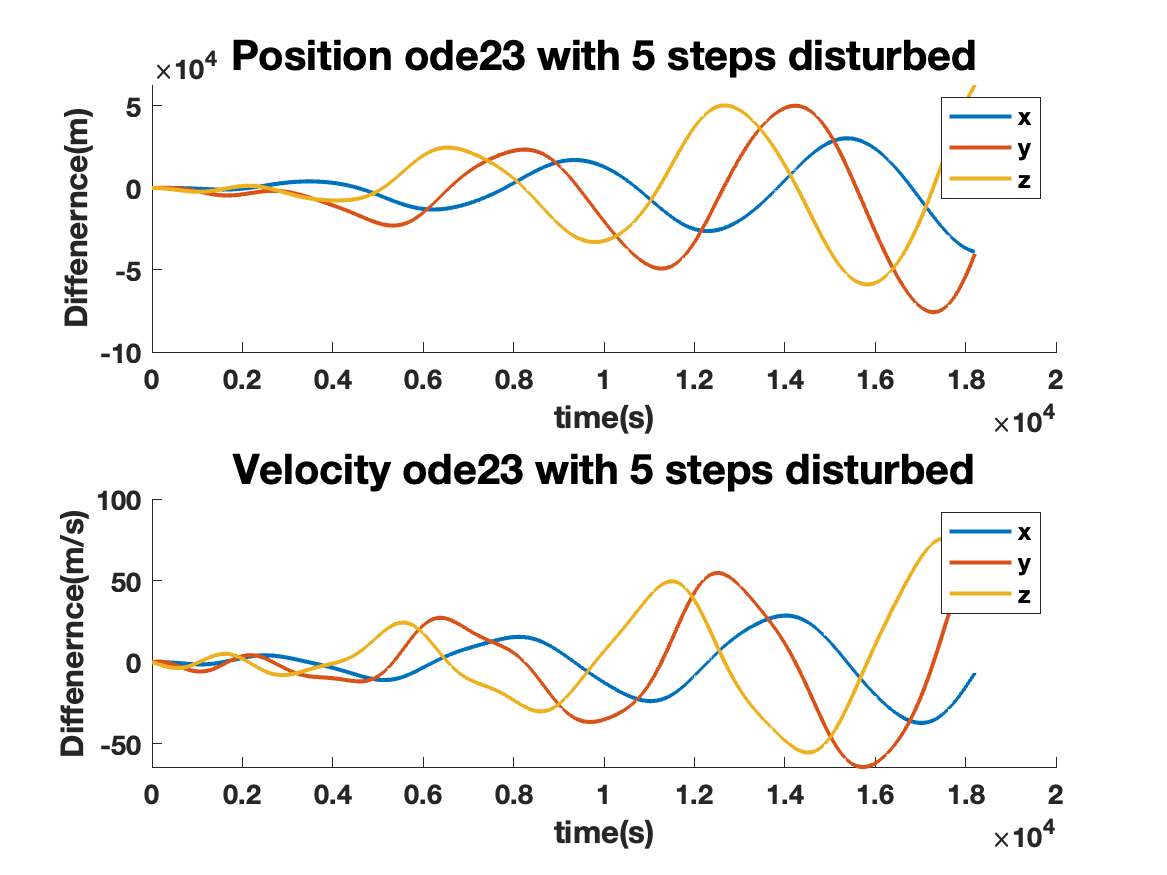
\includegraphics[width=1\textwidth]{./plots/ode23_5_yprime_d.png}
        \end{subfigure}
        \begin{subfigure}[b]{0.45\textwidth}
        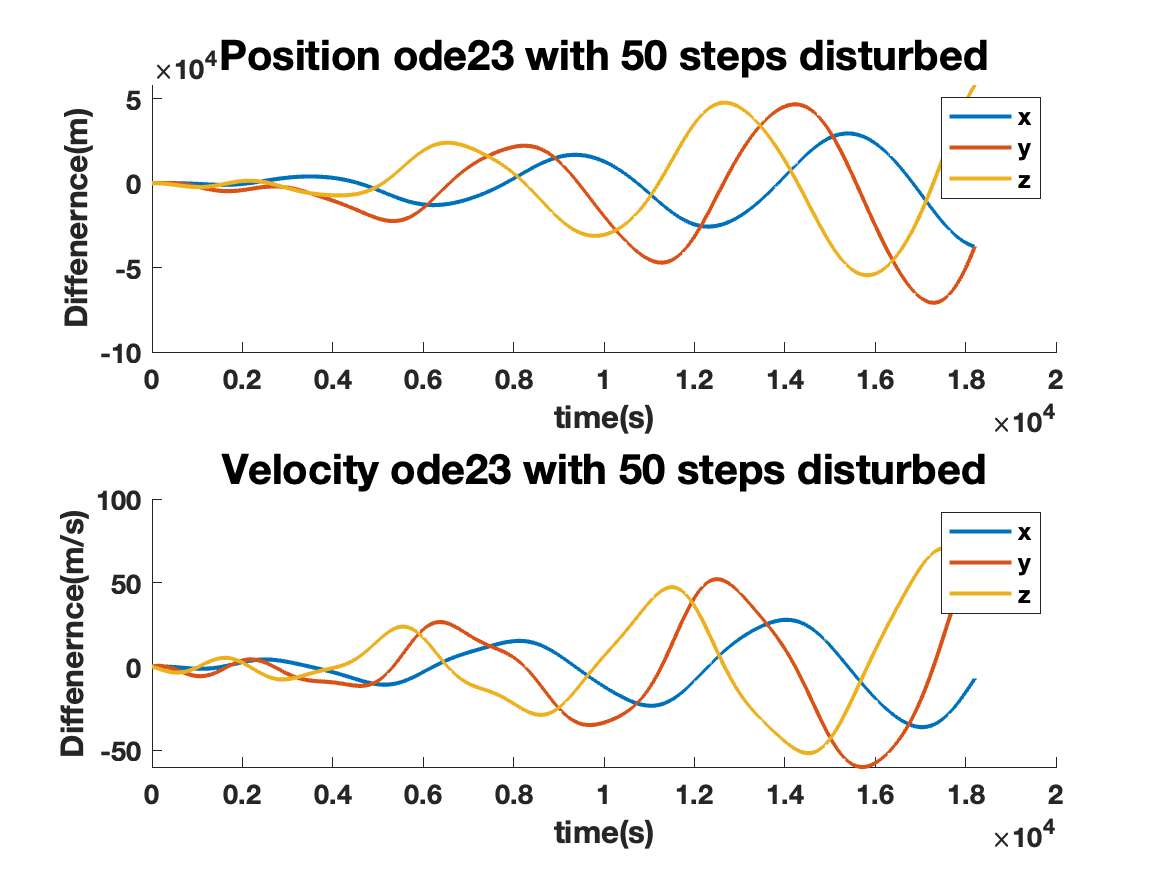
\includegraphics[width=1\textwidth]{./plots/ode23_50_yprime_d.png}
        \end{subfigure}
        \begin{subfigure}[b]{0.45\textwidth}
        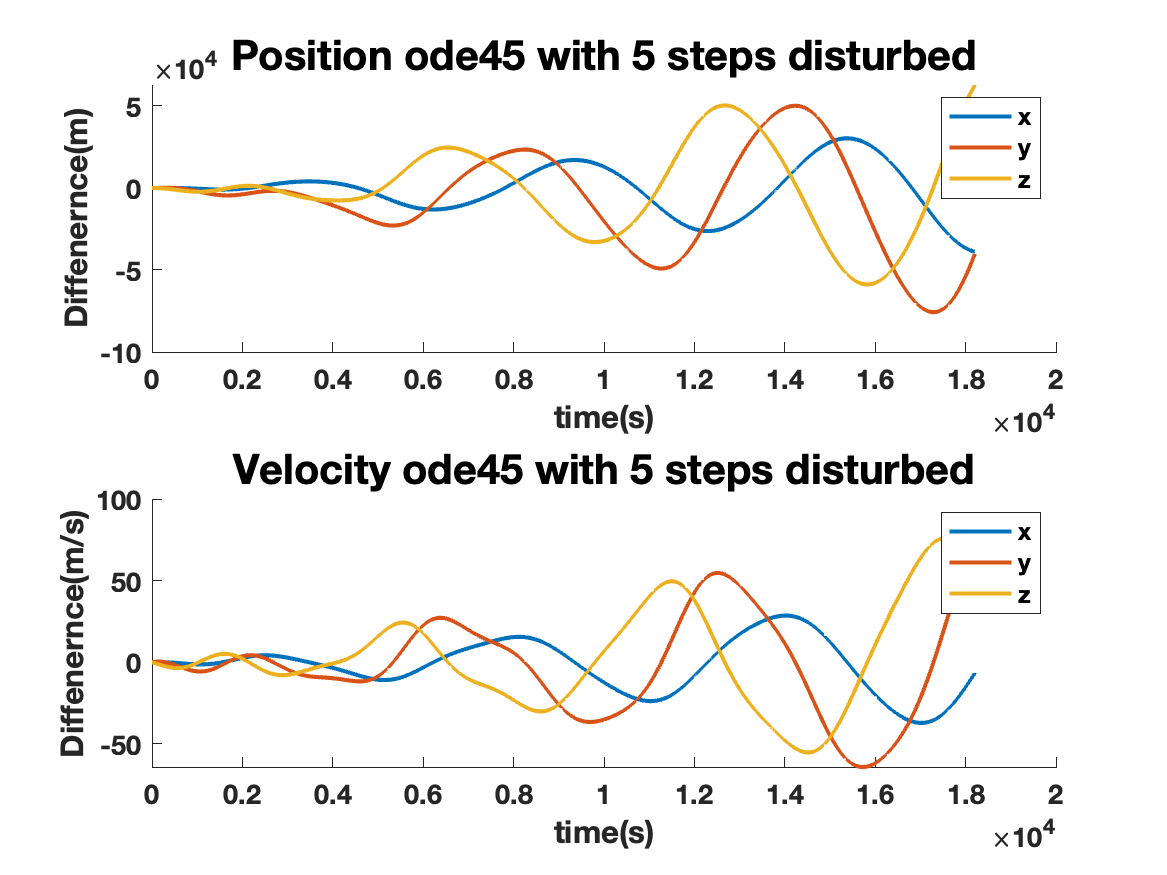
\includegraphics[width=1\textwidth]{./plots/ode45_5_yprime_d.png}
        \end{subfigure}
        \begin{subfigure}[b]{0.45\textwidth}
        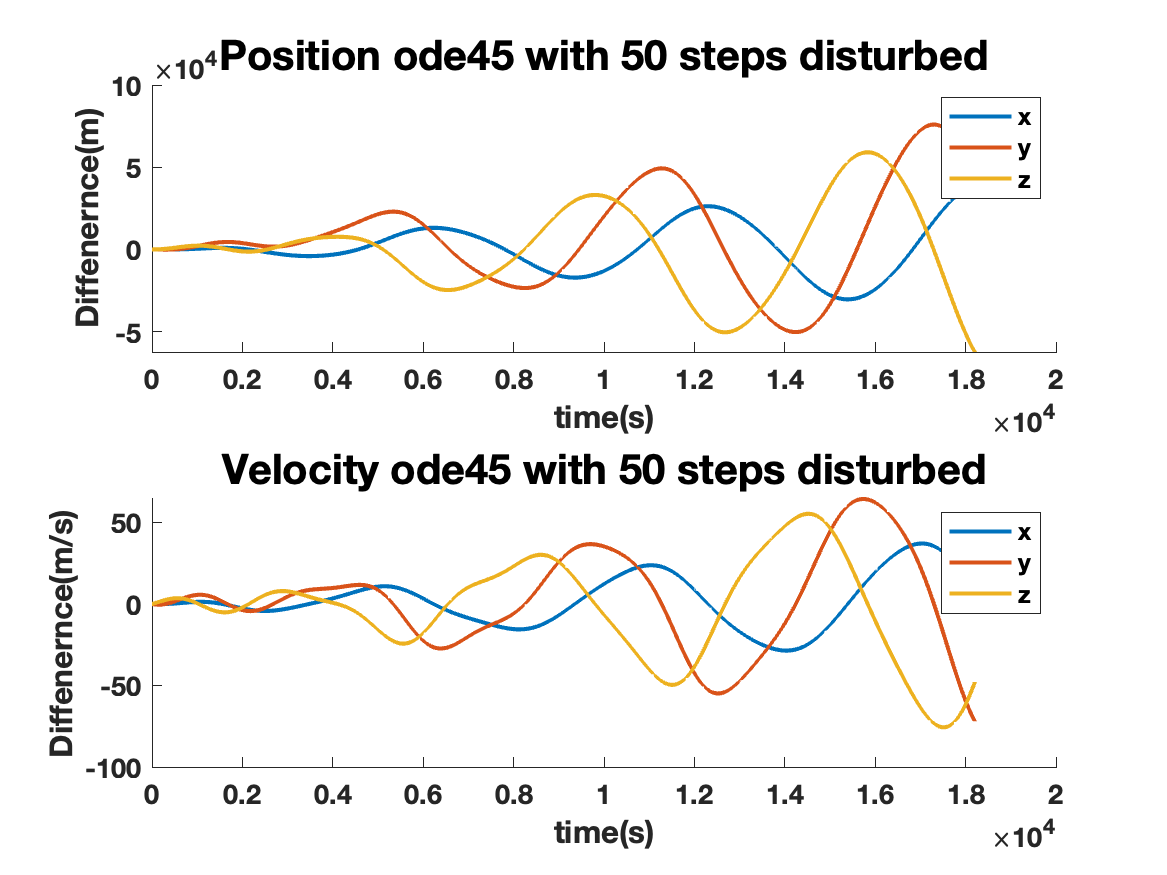
\includegraphics[width=1\textwidth]{./plots/ode45_50_yprime_d.png}
        \end{subfigure}
    \end{figure}
    In the figures, we can see that unlike the undisturbed orbit, the method od the numerical integration does not make a big difference, the results of both \textbf{ode23} and \textbf{ode45} are similar. 
    Compare to the undisturbed orbit, we can see that the difference between analytical solution and numerical integration is larger. For the \textbf{ode23} with step size of 5, the max. difference in position increases from 5m to about 50 km. For the \textbf{ode45} with step size of 5, the max. difference in position increases from less than 1mm to about 50 km. For the \textbf{ode23} with step size of 50, the max.\ difference in position increases from 5km to about 50 km. For the \textbf{ode45} with step size of 50, the max. difference in position increases from 0.2m to about 50 km. The difference in the velocity is also larger than the undisturbed orbit. The differences in undisturbed are all less than 1m/s except for the \textbf{ode23} with step size of 50, which is about 5m/s. The differences in the disturbed orbit are all larger than 1m/s, about 100m/s no mater which method and step size we use.
    \subsection*{In RSW frame}
    Analogous to the undisturbed orbit, we can also decompose the error in the RSW system. The results are shown in the following figures:
    \begin{figure}[H]
        \centering
        \begin{subfigure}[b]{0.45\textwidth}
        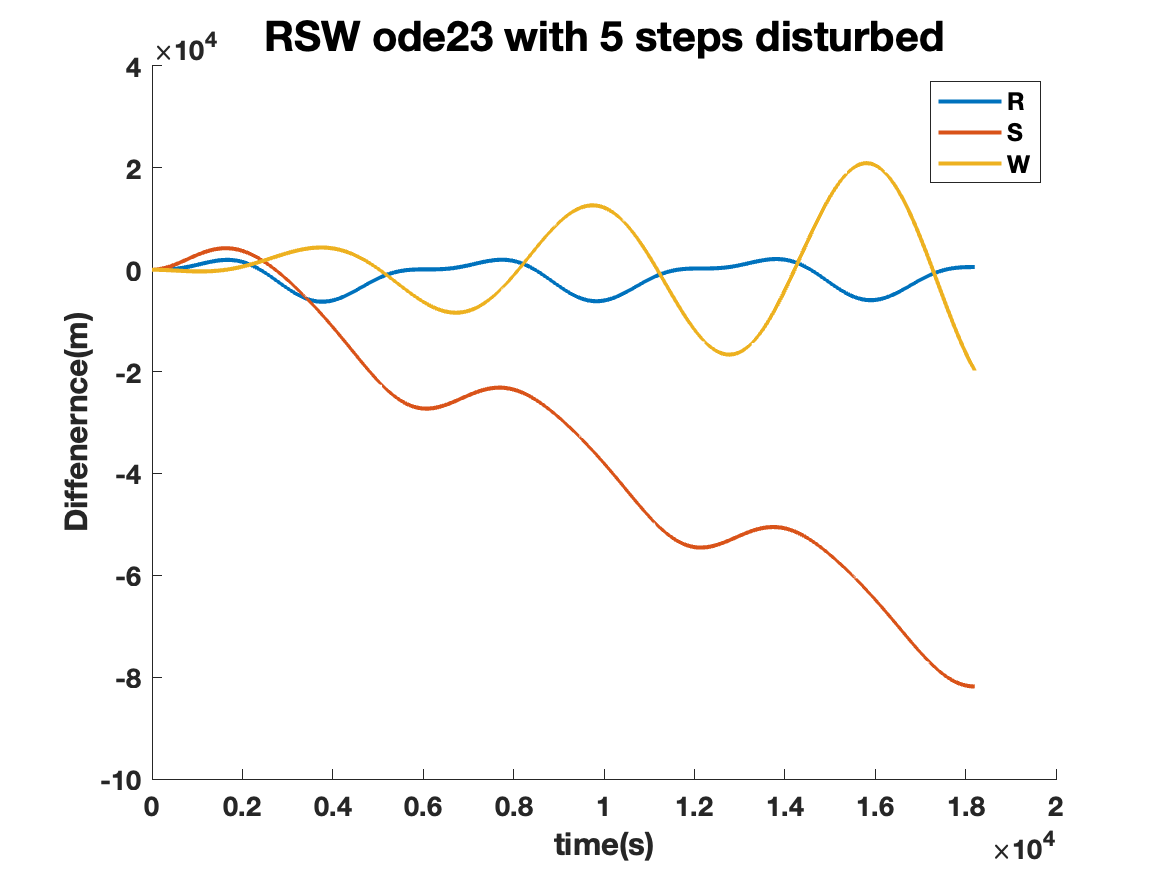
\includegraphics[width=1\textwidth]{./plots/ode23_5_yprime_d_RSW.png}
        \end{subfigure}
        \begin{subfigure}[b]{0.45\textwidth}
        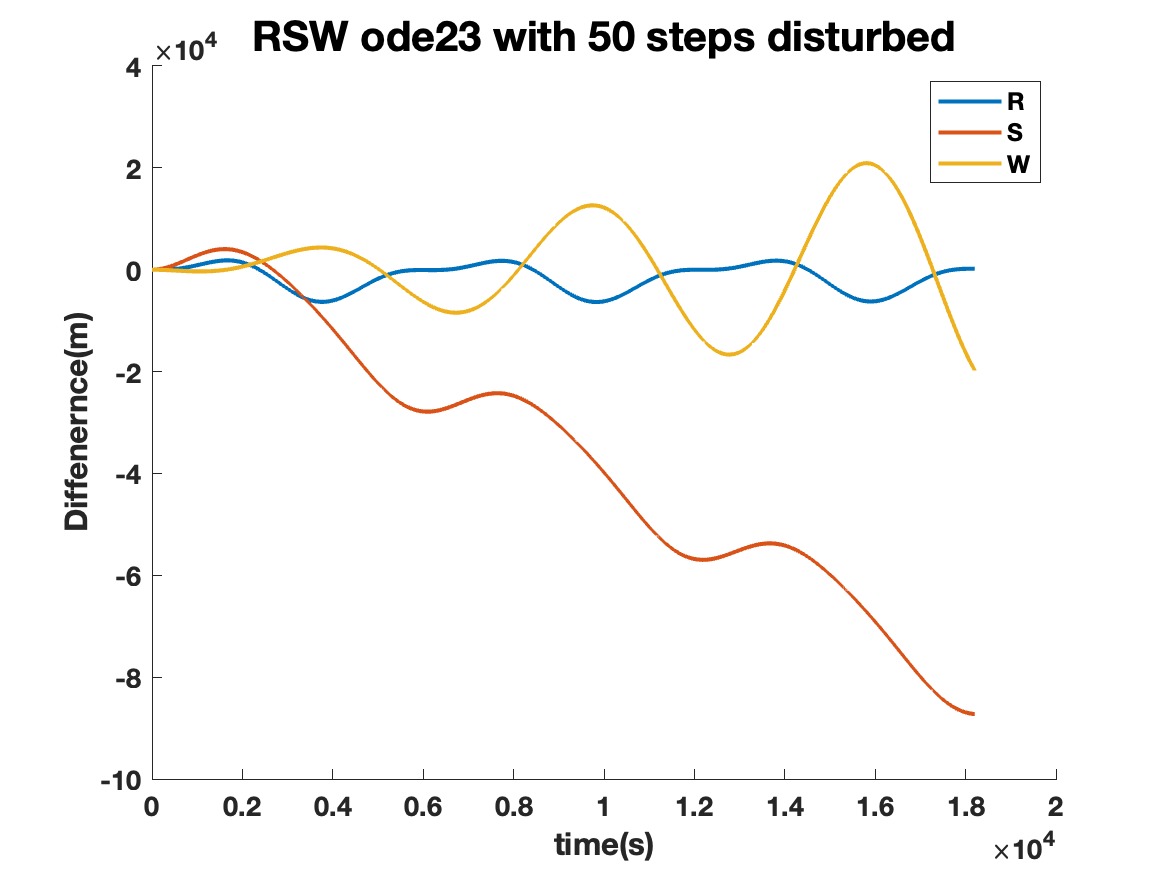
\includegraphics[width=1\textwidth]{./plots/ode23_50_yprime_d_RSW.png}
        \end{subfigure}
        \begin{subfigure}[b]{0.45\textwidth}
        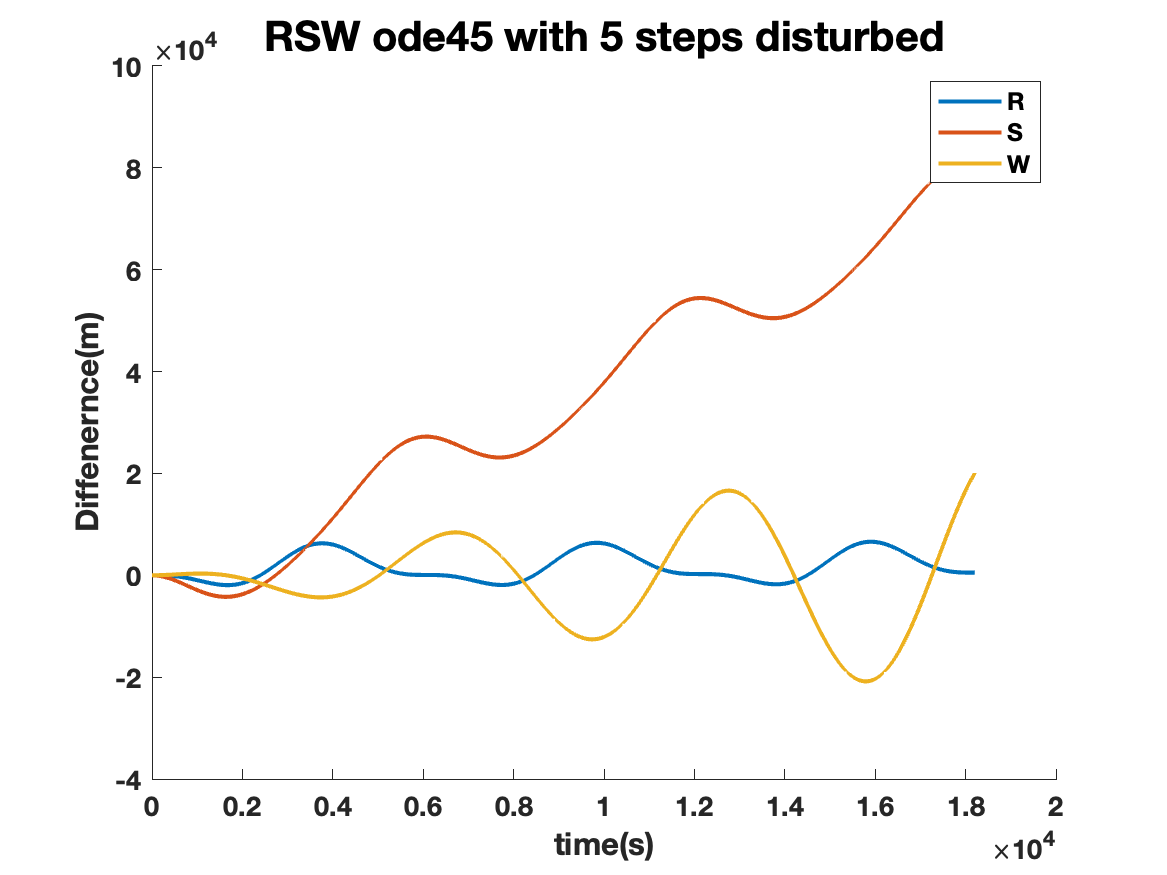
\includegraphics[width=1\textwidth]{./plots/ode45_5_yprime_d_RSW.png}
        \end{subfigure}
        \begin{subfigure}[b]{0.45\textwidth}
        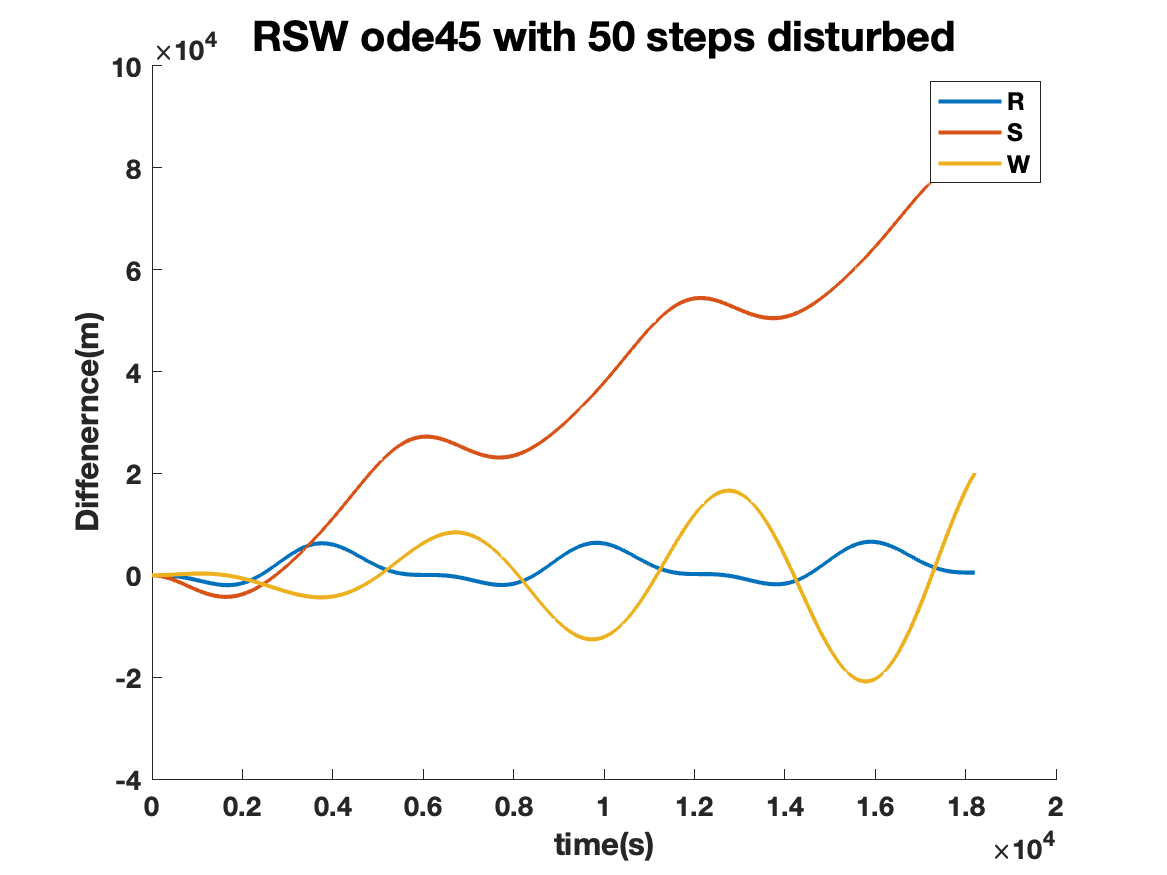
\includegraphics[width=1\textwidth]{./plots/ode45_50_yprime_d_RSW.png}
        \end{subfigure}
    \end{figure} 
    In the undisturbed case, we drawed a conclusion that the difference is mostly in the along-track (S) direction, which is still the case for the disturbed orbit. However, the difference in the radial (R) and cross-track (W) directions are also larger than the undisturbed orbit. The max.\ difference in the along-track (S) direction can reach 100km. The max.\ difference in the cross-track (W) direction can reach 10km. 
    The difference in the radial direction is larger than 100m, which is about 100 times larger than the undisturbed orbit. The difference in the cross-track direction is larger than 10km.
\section*{Own Implementation of the Numerical Integration}
Now we want to implement our own numerical integration function. A simple case is to use Euler method to solve the differential equation. The Euler method is given by:
\begin{align*}
    \textbf{y}_{n+1}=\textbf{y}_n+h\textbf{f}(t_n,\textbf{y}_n)
\end{align*}
A more precise method is the Runge-Kutta method. The Runge-Kutta 4th order method is given by:
\begin{align*}
    \textbf{y}_{n+1}&=\textbf{y}_n+\frac{h}{6}(k_1+2k_2+2k_3+k_4)\\
    k_1&=\textbf{f}(t_n,\textbf{y}_n)\\
    k_2&=\textbf{f}(t_n+\frac{h}{2},\textbf{y}_n+\frac{h}{2}k_1)\\
    k_3&=\textbf{f}(t_n+\frac{h}{2},\textbf{y}_n+\frac{h}{2}k_2)\\
    k_4&=\textbf{f}(t_n+h,\textbf{y}_n+hk_3)
\end{align*}
The results of the numerical integration with the Euler method and Runge-Kutta method are shown in the following figures:
\begin{figure}[H]
    \centering
    \begin{subfigure}[b]{0.45\textwidth}
    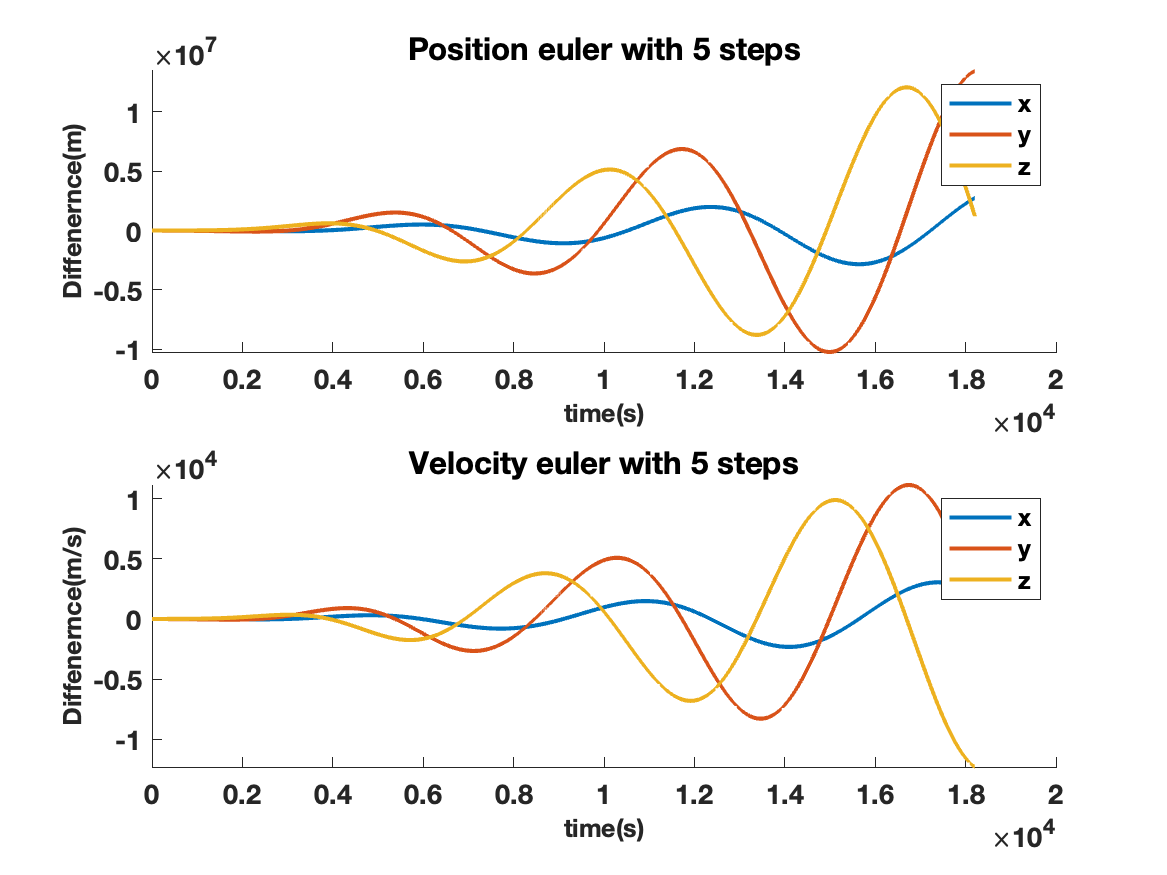
\includegraphics[width=1\textwidth]{./plots/euler_5_yprime.png}
    \end{subfigure}
    \begin{subfigure}[b]{0.45\textwidth}
    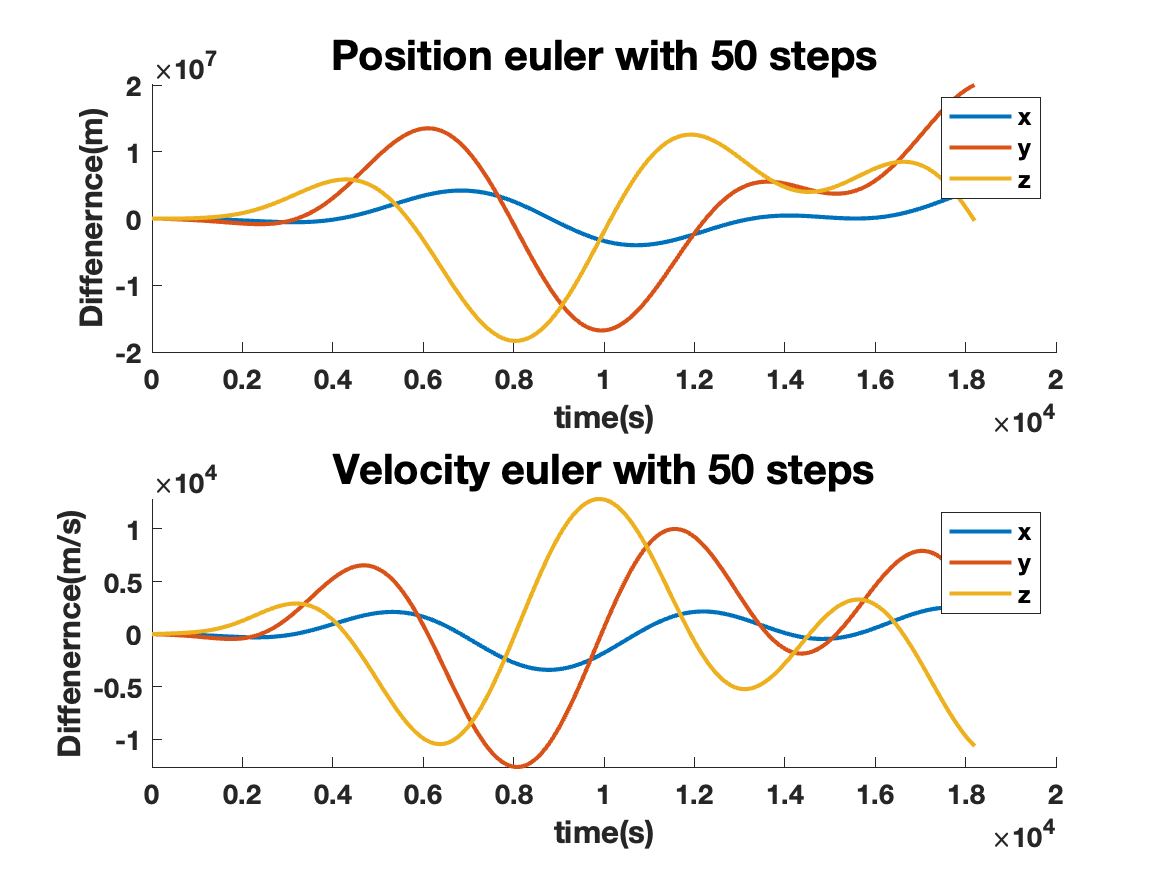
\includegraphics[width=1\textwidth]{./plots/euler_50_yprime.png}
    \end{subfigure}
    \begin{subfigure}[b]{0.45\textwidth}
    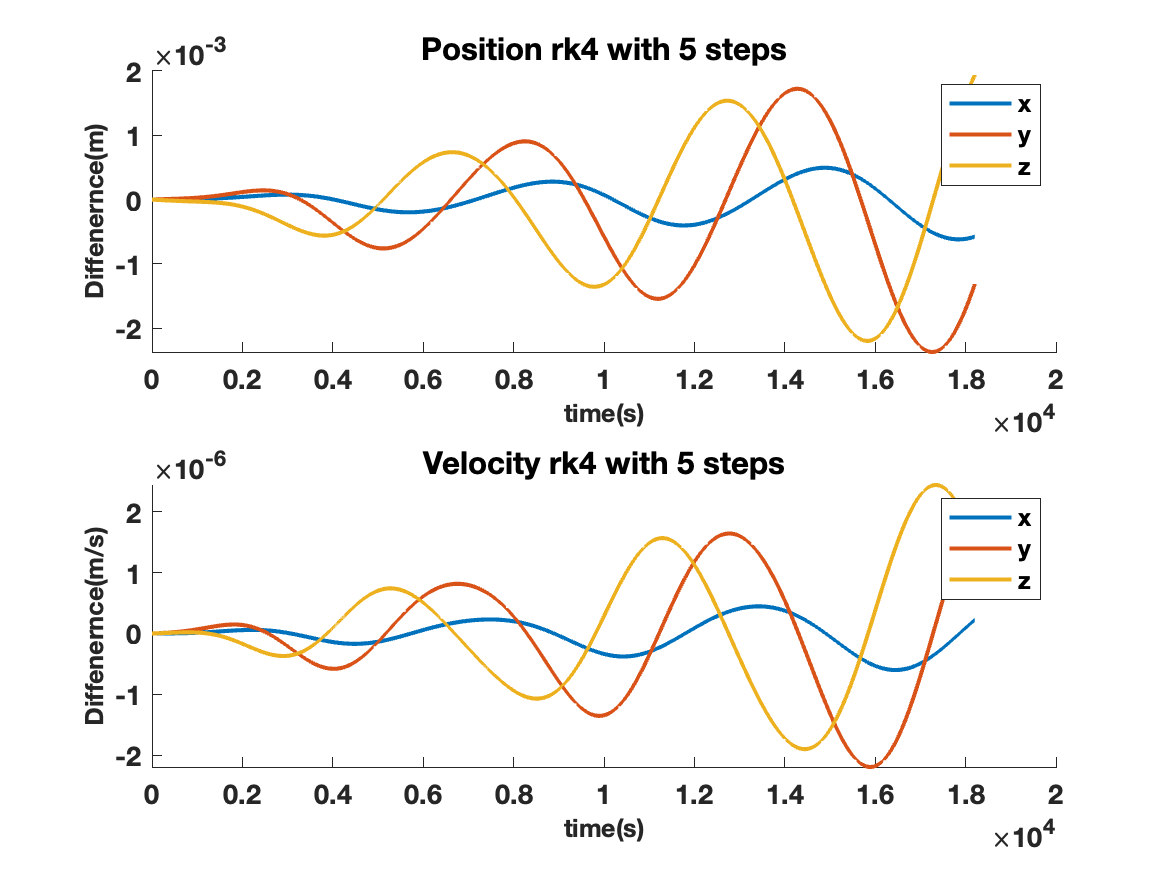
\includegraphics[width=1\textwidth]{./plots/rk4_5_yprime.png}
    \end{subfigure}
    \begin{subfigure}[b]{0.45\textwidth}
    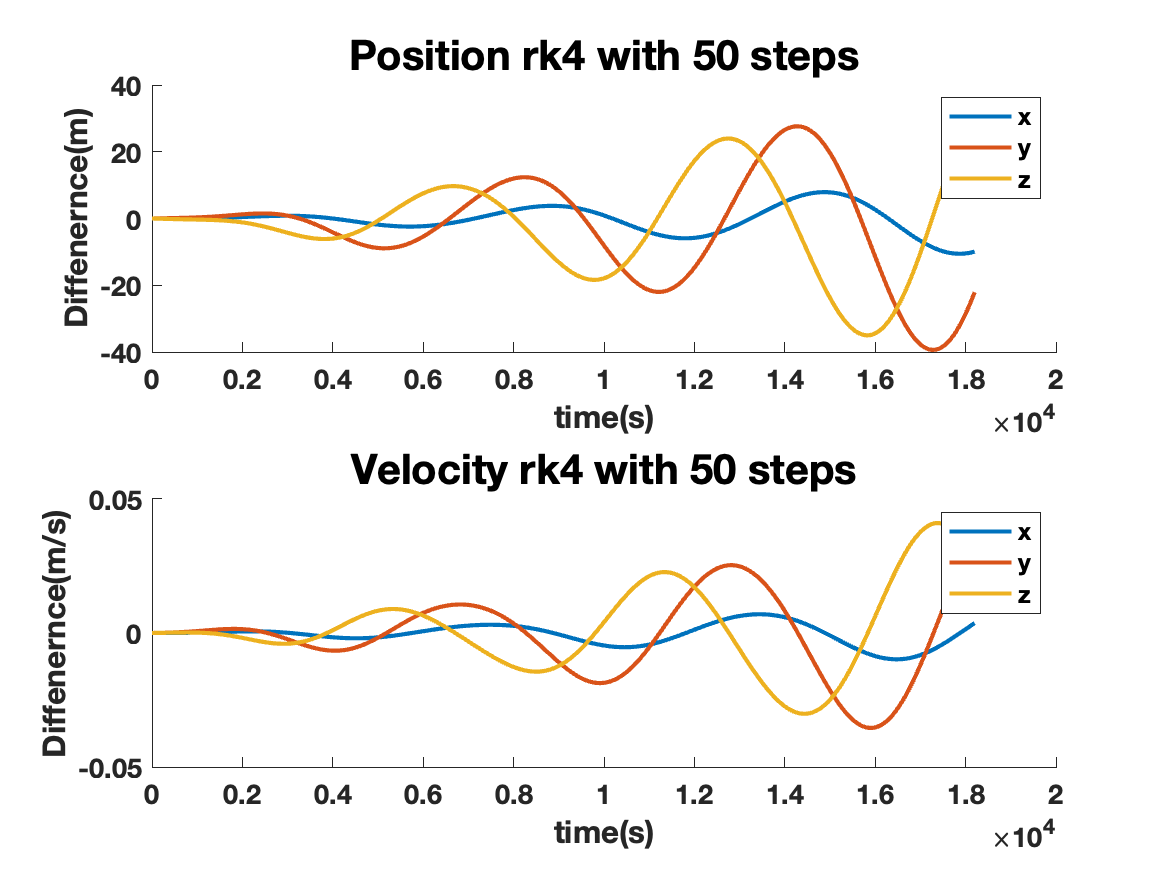
\includegraphics[width=1\textwidth]{./plots/rk4_50_yprime.png}
    \end{subfigure}
\end{figure}
From the formulas of Euler and Runge-Kutta method of order 4, we can determin that the results of rk4 should be much better than Euler method, because the Runge-Kutta method of order four requires four evaluations per step, whereas Euler method requires only one evaluation. And the results are as expected. We can see that even with a step size of 5, the position difference of Euler method can reach 1000km, which is about $10^10$ times larger than the Runge-Kutta method of order 4 with the same step size. 
For Runge-Kutta method of order 4, even with a large step size of 50, the largest position difference is still less than 40m. The velocity difference is less than 0.05m/s, which is a very high precision.
\end{document}